
\chapter{The simulator}
\label{chap:simul}

Afterwards, I worked on the simulator to know specificities of the simulator and realize the layer of communication.

\section{Specificity of the UML Model}

The Ciprian simulator simulate a UML model but this UML model need to have some specificities in the architecture and in the language.

\umld use 2 files to save a uml project. The first is named \textit{model.uml} it contains all UML elements and the declaration of UML diagrams. The second is named \textit{representation.aird}, it contains the specification of the graphical representation.

To work, the simulator need the \textit{model.uml} file. Moreover, this file need to contain some specifics features. It need a class \textbf{SUS} which contain the declaration of all other classes and all other classes need to have a State Machine diagram associated, as you can see on the figure \ref{fig:simulateur}.

\begin{figure}[h!]
  \centering
  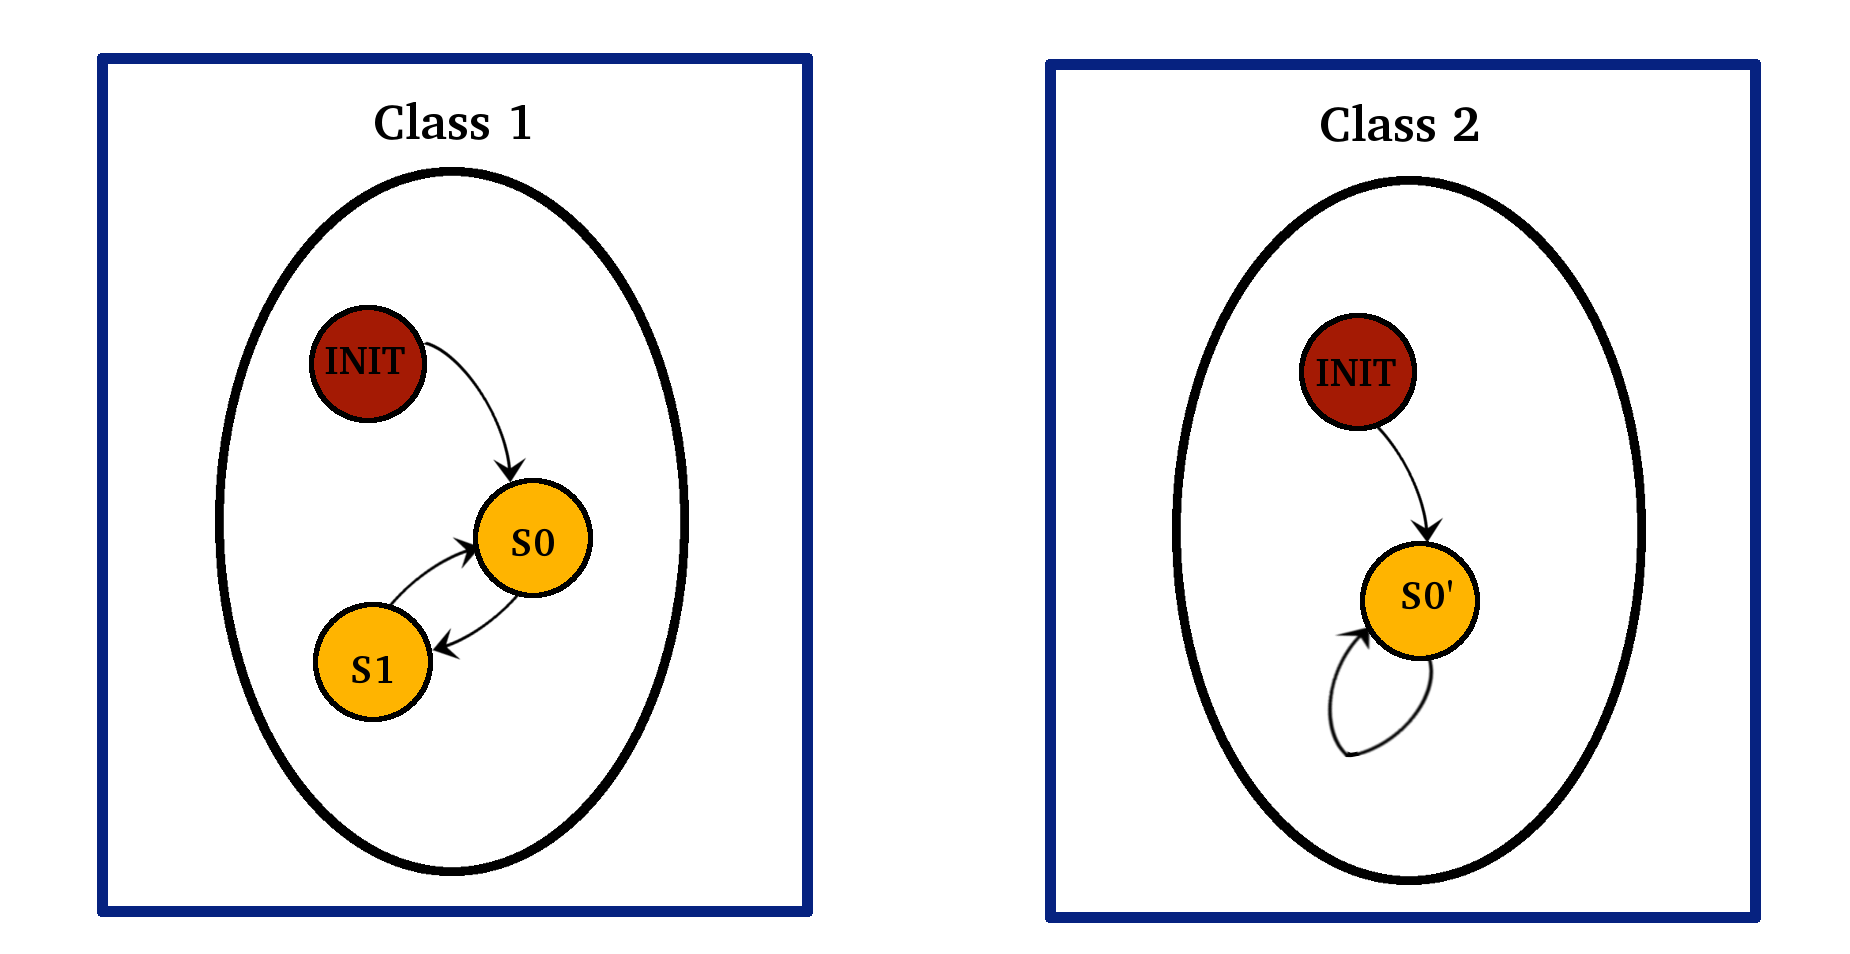
\includegraphics[width=\textwidth]{simulation}
  \caption{Representation of the most important elements for the simulator}
  \label{fig:simulateur}
\end{figure}

\section{Additions to Teodorov Simulator}

Then, I made some research on the code of the simulator. I realize that the simulator was not develop to communicate and notify any changing. So I change the code of the simulator to add an Observer pattern at the class \textit{SimulationModel} because this class is a controller of the simulator.

\begin{quotation}
<<The Observer pattern is a software design pattern in which an object, called the subject, maintains a list of its dependents, called observers, and notifies them automatically of any state changes, usually by calling one of their methods.>> \cite{wiki_pattern}
\end{quotation}


I used this pattern to notify the communication class of a changing.

\section{Communication}



The communication Layer was written in Java. As it was explain in the chapter before, the simulator and its layer were implemented by default inside the plugin. The main class of the plugin initiate the Simulator in a new thread and then there is only a communication enter the plugin and the simulator though the localhost loop by socket.

%In the chapter before, we have decided to put the simulator outside. However, . So I put the simulator and its layer in . However,

Moreover, to be sure that is possible to change the default simulator with an outside simulator I did some test where the thread is initiate by an other software, and that's work. % So for the rest of this report we consider that the simulator is outside the plugin because the comportment is the same.%, but the default simulator is in fact initiate by the plugin.






%%% Local Variables:
%%% mode: latex
%%% TeX-master: "../rapport_de_base"
%%% End:
